\documentclass[12pt,twoside, draft]{article}
\usepackage{weiiszablon}
\author{Sławomir Zdunek}
\studentID{EF-177192}
\title{Symulacja fizyczna ciał sztywnych}
\titleEN{Rigid body physics simulation}
\newcommand{\rodzajPracyNo}{1}
\supervisor{dr hab. inż. Maciej Kusy prof. Prz}
\supervisorEN{Prof. Maciej Kusy, DSc Eng} % CHECK
\abstract{Treść streszczenia po polsku} % TODO
\abstractEN{Treść streszczenia po angielsku}
\keywords{fizyka, symulacja, dynamika, kolizje}
\keywordsEN{physics, simulation, dynamics, collisions.}

\begin{document}

\maketitle

\blankpage
\tableofcontents
\clearpage
\blankpage

\section{Wstęp}
% Aplikacje: MuJoCo, Blender,  VistaKine
%https://www.blender.org
%https://github.com/google-deepmind/mujoco
%https://www.vistakine.com/playground
Współczesny rynek oprogramowania oferuje wiele narzędzi umożliwiających modelowanie trójwymiarowe, symulację zjawisk fizycznych oraz analizę ruchu obiektów.
Jedną z najpopularniejszych aplikacji implementującej symulowanie dynamiki ciał jest Blender\cite{blender}. 
Jest to bardzo rozbudowna, otwartoźródłowa aplikacja wykorzystywana głównie do modelowania 3D, natomiast daje możliwość symulowania fizyki tworzonych scen.


adsfkljasdfjk
Wytyczne:
Wstęp nie może składać się z podrozdziałów; powinien składać się z następujących akapitów:
 I akapit: w zależności od tematyki pracy: ogólny stan rynku. Przykład: jeżeli praca polega
na stworzeniu aplikacji, pierwszy akapit ma opisać stan rynku podobnych programów
(dostępnych w chwili obecnej). Na każdą aplikację należy poświęcić 4-5 zdań (podając
odnośniki do literatury). Uwaga: te właśnie aplikacje zostaną szczegółowo omówione
w następnym rozdziale. W akapicie powinno znaleźć się jak najwięcej odniesień do
literatury.
 II akapit: główne cele pracy, cele dodatkowe. Wyszczególnienie celów w omawianym
akapicie powinno przyjąć postać: "Głównym celem pracy jest opracowanie...". Jeżeli
występuje kilka celów, można je wypunktować.
 III akapit: Struktura pracy jest następująca: w Rozdziale 1 dokonano szczegółowej
charakterystyki porównawczej... Rozdział 2 opisuje... W Rozdziale 3 przedstawiono.
Rozdział ostatni podsumowuje pracę.

Rozdział 2. Szczegółowy opis aplikacji/urządzenia/układu
W niniejszym rozdziale przedstawiono wszystkie moduły jakie zostały zaimplementowane
w aplikacji... Są to Moduł 1, Moduł 2, Moduł 3 ...
2.1. Moduł 1
Pełne omówienie Modułu 1. Liczba stron do uzgodnienia z opiekunem.
Katedra Podstaw Elektroniki
Wytyczne dotyczące pisania i formatowania treści pracy dyplomowej
2.2. Moduł 2
Pełne omówienie Modułu 2. Liczba stron do uzgodnienia z opiekunem.
2.3. Moduł 3
Pełne omówienie Modułu 3. Liczba stron do uzgodnienia z opiekunem

\section{Technologie}
Rozdział opisuje środowisko programistyczne, język programowania ... jakie zostały
wykorzystane przez autora podczas tworzenia pracy... W tej części pracy przedstawiono
również programową implementację wybranych modułów programu. Liczba stron do
uzgodnienia z opiekunem.
\subsection{Środowisko programistyczne}
Omówienie
\subsection{Języki programowania}
Omówienie
3.3. Implementacje modułów
\subsubsection{Implementacja modułu X}
Opis modułu X, zasada działania (algorytm), kody źródłowe ujęte w ramki, kolorowa składnia
(podpis jako Listing 3.1....), omówienie kodu źródłowego. Najlepiej opisać moduł, który
sprawił autorowi najwięcej trudności.
\subsubsection{Implementacja modułu Y}
Opis modułu Y, zasada działania (algorytm), kody źródłowe ujęte w ramki, kolorowa składnia
(podpis jako Listing kontynuacja numerowania), omówienie kodu źródłowego. Najlepiej
opisać moduł, który sprawił autorowi najwięcej trudności.
\subsubsection{Implementacja modułu Z}
Opis modułu Z, zasada działania (algorytm), kody źródłowe ujęte w ramki, kolorowa składnia
(podpis jako Listing kontynuacja numerowania), omówienie kodu źródłowego. Najlepiej
opisać moduł, który sprawił autorowi najwięcej trudności

\section{Wnioski}
Rozdział wnioski nie może składać się z podrozdziałów; powinien składać się z takich
samych akapitów jak Wstęp, ale napisanych w czasie przeszłym i inaczej sformułowanych:

I akapit: w zależności od tematyki pracy: ogólny stan rynku.

II akapit: główne cele pracy (podkreślić, że zostały zrealizowane) .

III akapit: nowe ujęcie w zakresie pracy: Wyszczególnienie nowego ujęcia w omawianym
akapicie można przyjąć postać: "Do pracy wprowadzono następujące nowe
rozwiązania..." lub "Elementem nowości wprowadzonym do pracy jest..." lub „Nowym
ujęciem tematyki poruszanej w pracy jest …”

IV akapit: podczas realizacji pracy, autor napotkał na kilka problemów; wymienić dwa,
trzy i w kilku zdaniach napisać jak każdy z nich został rozwiązany

V akapit: "Praca napisana jest w formie pozwalającej na jej rozbudowę." Tutaj trzeba
dodać, jakie elementy czy moduły mogłyby (według autora) uatrakcyjnić pracę.
Wymienić dwa, trzy i krótko opisać.

\cleardoublepage
\addcontentsline{toc}{section}{Literatura}

\begin{thebibliography}{4}
\bibitem{blender} https://docs.blender.org/manual/en/5.3/getting\_started/about/index.html Dostęp 12.11.2026.
\bibitem{blenderFeat} https://www.blender.org/features/ Dostęp 12.11.2026.
\bibitem{blenderSim} https://www.blender.org/features/simulation/ Dostęp 12.11.2026.
\bibitem{blenderSkrypt} https://www.blender.org/features/scripting/ Dostęp 12.11.2026.
\bibitem{deepMind} https://www.deepmind.com/ Dostęp 12.11.2026.
\bibitem{MuJoCo} https://github.com/google-deepmind/mujoco Dostęp 12.11.2026.
\bibitem{MuJoCoDemo} https://mujoco.org/ Dostęp 12.11.2026.
\bibitem{Rapier} https://rapier.rs/ Dostęp 12.11.2026. 
\bibitem{RapierDocs} https://rapier.rs/docs/ Dostęp 12.11.2026.
\bibitem{RapierDemo} https://rapier.rs/demos/ Dostęp 12.11.2026.
\bibitem{RapierDemo2D} https://rapier.rs/demos/\#2d Dostęp 12.11.2026.
\end{thebibliography}

% https://matthias-research.github.io/pages/tenMinutePhysics/09-xpbd.pdf
% https://matthias-research.github.io/pages/publications/PBDBodies.pdf
% https://matthias-research.github.io/pages/tenMinutePhysics/24-morton.pdf
% https://matthias-research.github.io/pages/tenMinutePhysics/11-hashing.pdf
% https://www.medien.ifi.lmu.de/lehre/ss10/ps/Ausarbeitung\_Beispiel.pdf
% https://winter.dev/articles/epa-algorithm/

\clearpage
\makesummary
\end{document} 

% \begin{figure}[ht]%
%  \centering%
%  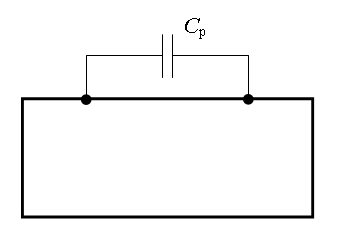
\includegraphics[width=6cm]{figures/fig1.png}%
%  \caption{Tytuł rysunku, rozmiar 11 pkt, pojedyncza interlinia, akapit wyśrodkowany, bez wcięcia pierwszego wiersza. Na końcu tytułu rysunku/tabeli nie stawia się kropki [8]}%
%  \label{Fig:schemat}%
% \end{figure}

% \begin{lstlisting}[language=Matlab,caption=Listing programu Matlab,label={KodMatlab1}]
% i = 1
% p = 3
% for i = 1:10
%     if i > 3
%         i=i+p
%     else 
%         i=i+1
%     end
% end
% \end{lstlisting}

% \lstinputlisting[language={[ANSI]C},inputencoding=utf8/cp1250,firstline=2,lastline=6,breaklines=true,numbers=left,frame=hnone,caption={Polskie znaki diakrytyczne w kodzie},label={lst:plchr}]{auxiliary/start.c}
